\documentclass{exam}
\usepackage[utf8]{inputenc}
\usepackage{lmodern}
\usepackage{microtype}

% \usepackage[parfill]{parskip}
\usepackage[dvipsnames]{xcolor}
\usepackage{amsmath}
\usepackage{amsfonts}
\usepackage{amsthm}
\usepackage{siunitx}
\DeclareSIUnit\year{yr}
\DeclareSIUnit\foot{ft}
\DeclareSIUnit\litre{\liter}

\usepackage{skull}

\usepackage{pgfplots}
\usepgfplotslibrary{polar}
\pgfplotsset{compat=1.11}
\usepgfplotslibrary{statistics}
\usepackage{graphicx}
\usepackage{sidecap}
\sidecaptionvpos{figure}{c}
\usepackage{float}
\usepackage{gensymb}
\usepackage{tkz-euclide}
\usetkzobj{all}
\usepackage{commath}
\usepackage{hyperref}
\usepackage{enumitem}
\usepackage{wasysym}
\usepackage{multicol}
\usepackage{mathtools}
\usepackage{tcolorbox}
\usepackage{tabularx}
\usepackage[version=4]{mhchem}
\usepackage{changepage}
\usepackage{listings}
\lstset{basicstyle=\ttfamily\linespread{0.8}\small}

\renewcommand*{\thefootnote}{\fnsymbol{footnote}}

\newtheorem*{thm}{Theorem}
\newtheorem*{iden}{Identity}
\newtheorem*{lemma}{Lemma}
\newtheorem{obs}{Observation}
\theoremstyle{definition}
\newtheorem*{defn}{Definition}
\newtheorem*{ex}{Example}
\newtheorem{con}{Construction}
\newtheorem*{alg}{Algorithm}

\newtheoremstyle{break}
  {\topsep}{\topsep}%
  {\itshape}{}%
  {\bfseries}{}%
  {\newline}{}%
\theoremstyle{break}
\newtheorem*{bthm}{Theorem}

% russian integral
\usepackage{scalerel}
\DeclareMathOperator*{\rint}{\scalerel*{\rotatebox{17}{$\!\int\!$}}{\int}}

% \DeclareMathOperator*{\rint}{\int}

\pgfplotsset{vasymptote/.style={
    before end axis/.append code={
        \draw[densely dashed] ({rel axis cs:0,0} -| {axis cs:#1,0})
        -- ({rel axis cs:0,1} -| {axis cs:#1,0});
    }
}}

% \pointsinrightmargin
\boxedpoints
\pointname{}

\newcommand{\questioA}{\question[\texttt{\textbf{\color{Cerulean} A}}]}
\newcommand{\questioM}{\question[\texttt{\textbf{\color{PineGreen} M}}]}
\newcommand{\questioE}{\question[\texttt{\textbf{\color{WildStrawberry} E}}]}
\newcommand{\questioS}{\question[\texttt{\textbf{\color{Goldenrod} S}}]}
\newcommand{\questioO}{\question[\texttt{\textbf{\color{BurntOrange} O}}]}

\newcommand{\parA}{\part[\texttt{\textbf{\color{Cerulean} A}}]}
\newcommand{\parM}{\part[\texttt{\textbf{\color{PineGreen} M}}]}
\newcommand{\parE}{\part[\texttt{\textbf{\color{WildStrawberry} E}}]}
\newcommand{\parS}{\part[\texttt{\textbf{\color{Goldenrod} S}}]}
\newcommand{\parO}{\part[\texttt{\textbf{\color{BurntOrange} O}}]}

\newcommand{\subparA}{\subpart[\texttt{\textbf{\color{Cerulean} A}}]}
\newcommand{\subparM}{\subpart[\texttt{\textbf{\color{PineGreen} M}}]}
\newcommand{\subparE}{\subpart[\texttt{\textbf{\color{WildStrawberry} E}}]}
\newcommand{\subparS}{\subpart[\texttt{\textbf{\color{Goldenrod} S}}]}
\newcommand{\subparO}{\subpart[\texttt{\textbf{\color{BurntOrange} O}}]}

\newcommand{\mainHeader}[2]{\section*{NCEA Level 2 Mathematics\\#1. #2}}
\newcommand{\mainHeaderHw}[2]{\section*{NCEA Level 2 Mathematics (Homework)\\#1. #2}}
\newcommand{\seealso}[1]{\begin{center}\emph{See also #1.}\end{center}}
\newcommand{\drills}[1]{\begin{center}\emph{Drill problems: #1.}\end{center}}
\newcommand{\basedon}[1]{\begin{center}\emph{Notes largely based on #1.}\end{center}}

\usepackage[normalem]{ulem}
\usepackage{venndiagram}
\begin{document}

\mainHeader{22}{Probability and Risk}

\subsection*{Basic probability}

Suppose we are performing an experiment where the outcome is uncertain. Some examples
of such experiments include:-
\begin{itemize}
  \item Flipping a coin.
  \item Measuring rainfall.
  \item Determining the sex of a newborn child.
  \item Checking the outcome of a sporting event.
\end{itemize}

The set of possible outcomes of an experiment is called the \emph{sample space}. The
sample space of the first experiment above, that of flipping a coin, is
\begin{displaymath}
  S_\text{coin flip} = \{ H, T \}.
\end{displaymath}

The \emph{probability} of a given outcome is the proportion of times that we would expect
an experiment to give a particular outcome if we run the experiment multiple times. We
write $ P(\text{outcome}) $ for the probability of a particular outcome.

For example, $ P(H) = 0.5 $ because, if we were to flip a coin many times, we would expect
half the tosses to result in an outcome of $ H $.

A probability must lie between $ 0 $ and $ 1 $ inclusive (because it makes no sense for an outcome to happen in 200\% of the
experimental runs).

There are a couple of ways to determine the probability of something. We either find a probability experimentally,
by doing an experiment a bunch of times, or we do it theoretically, by counting outcomes.

\begin{itemize}
  \item To determine a probability experimentally --- based on empirical evidence:
        \begin{displaymath}
          P(A) = \frac{\text{number of times $A$ happened}}{\text{number of times the experiment ran}}.
        \end{displaymath}
  \item If there are $ n $ ways for an outcome $ A $ to occur, and each way is equally likely, then
        \begin{displaymath}
          P(A) = \frac{\text{number of ways $A$ could happen}}{\text{number of ways any outcome could happen}}.
        \end{displaymath}
\end{itemize}

We have some rules to calculate with probabilities. If $ A $ and $ B $ are two possible outcomes,
I will write $ P(A \vee B) $ for the probability that $ A $ \emph{or} $ B $ happens,\footnote{By `$ A $ or $ B $
happens', I mean that one of $ A $, $ B $, or both $ A $ and $  B$ happens.} and $ P(A \wedge B) $ for the
probability that $ A $ \emph{and} $ B $ happens.

If the total sample space consists of $ n $ outcomes, $ S = \{A_1, A_2, ..., A_n\} $, then
\begin{displaymath}
  P(A_1 \vee A_2 \vee \cdots \vee A_n) = 1.
\end{displaymath}
In other words, there is a probability of $ 1 $ --- absolute certainty --- that there will be an outcome. Either
heads or tails must be flipped.\footnote{Yes, it is possible for a coin to land on its rim. I am assuming an infinitely
thin coin, or maybe a counter.}

Two outcomes $ A $ and $ B $ are said to be \emph{mutually exclusive} if they can never happen at the same time;
in other words, if $ P(A \wedge B) = 0 $. To take the example of flipping a coin, heads and tails are mutually
exclusive outcomes.

If two events $ A $ and $ B $ are mutually exclusive, then $ P(A \vee B) = P(A) + P(B) $: the number of times
that $ A $ or $ B $ happens is the sum of the number of times that $ A $ or $ B $ happens.

Suppose $ A $ is an outcome. Then `not $ A $' is an outcome as well. Further, $ A $ and not $ A $ are mutually
exclusive; and they make up an entire sample space for our experiment because if we do the experiment, then either
$ A $ is the outcome or it isn't. Hence $ P(A) + P(\text{not } A) = 1 $, and thus $ P(\text{not } A) = 1 - P(A) $.
To save \sout{chalk} typing, I will write $ \neg A $ for `not $ A $'.

Now, suppose two events $ A $ and $ B $ are \emph{not} mutually exclusive: so it is possible for $ A \wedge B $ to
be an outcome of an experiment. We want to show that $ P(A \vee B) = P(A) + P(B) - P(A \wedge B) $.

\begin{proof}[Proof 1: via Venn diagram]
  If we draw a Venn diagram showing the $ P(A \wedge B) $, we end up with:

  \begin{center}
    \begin{venndiagram2sets}[labelAB=$A \wedge B $, radius=2.4cm, overlap=1.5cm]
    \end{venndiagram2sets}
  \end{center}
  So we see that $ P(A \vee B) = P(A) + P(B) - P(A \wedge B) $.
\end{proof}

\begin{proof}[Proof 2: algebraic]
  First, see that $ A \vee B = A \vee (B \wedge \neg A) $, where these events are mutually exclusive. (Either $ A $
  happens --- which could include $ A $ and $ B $ happening --- or $ B $ happens but not $ A $). We can apply the rule
  from above: $ P(A \vee B) = P(A) + P(B \wedge \neg A) $.

  Now, note that $ B = (B \wedge A) \vee (B \wedge \neg A) $ ($ B $ happens whenever $ B $ and $ A $ both happen, or
  when $ B $ happens without $ A $), where again the events are mutually exclusive. Hence $ P(B) = P(A \wedge B) + P(B \wedge \neg A) $.
  So we have both of the following:
  \begin{gather*}
    P(A \vee B) = P(A) + P(B \wedge \neg A)\\
    P(B) = P(A \wedge B) + P(B \wedge \neg A).
  \end{gather*}
  From the second, $ P(B \wedge \neg A) = P(B) - P(A \wedge B) $; and substituting into the first, $ P(A \vee B) = P(A) + P(B) - P(A \wedge B) $.
\end{proof}

Two outcomes $ A $ and $ B $ are called \emph{independent} if the the occurrence or nonoccurrence of one
does not affect the likelihood of occurrence or nonoccurence of the other. For example, the events `it will rain tomorrow in Brazil'
and `the sun will rise at 5:30 am in New Zealand' are independent.\footnote{One hopes. It is possible to imagine scenarios where they
turn out not to be independent --- for example, suppose a crazed supervillain from Dunedin decides he will blow up the country if it
rains in Brazil tomorrow.}

Suppose I flip a coin and roll a die. By drawing a table (see below) and counting the outcomes, I find that there
is a 1 in 12 chance ($ P = \frac{1}{12} $) that I flip a heads and roll a 6.

\begin{center}
  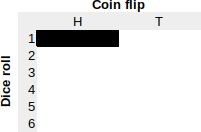
\includegraphics[width=0.2\textwidth]{independence}
\end{center}

Further experimentation should convince you that, if $ A $ and $ B $ are independent, then $ P(A \wedge B) = P(A) P(B) $.

If two events are \emph{not} independent, we can't apply this rule. We \emph{can} discuss the probability that $ A $ occurs
given $ B $: if $ P(A | B) $ is the probability that $ A $ occurs if it is known that $ B $ has occurred, then $ P(A \wedge B) = P(B) P(A | B) $.

\subsection*{Relative risk}

Suppose we are conducting a medical trial, and we want to examine the differences in outcomes between two groups. For example,
suppose we survey 1000 people and we split them up into two groups according to whether they smoke. We find that 200 people
are smokers, and 800 are non-smokers. We then track them for the rest of their lives, and find that twenty of the smokers
developed lung cancer, and four of the non-smokers did.

\begin{tabular}{|r|c|c|c|}\hline
  & \textbf{Smoker} & \textbf{Non-smoker} & \textbf{Total}\\\hline
  \textbf{Cancer} &20&4&24\\\hline
  \textbf{Non-cancer} &180& 796 & 976 \\\hline
  \textbf{Total} &200&800&1000\\\hline
\end{tabular}

We can't directly compare the actual numbers of cancer sufferers, 4 versus 20, to show that lung cancer and smoking are linked
because the sizes of the cohorts are different: it makes no sense to say that smokers are five times ($ 20/4$) more likely to get cancer
on the basis of these figures. To solve this problem, we want to calculate the risks (probabilities) of lung cancer in the presence
of smoking versus non-smoking, and then compare these.

We learn that, given a person is a smoker, they have a $ 20/200 = 0.1 $ probability of developing
lung cancer. On the other hand, if a person does not smoke, they have a $ 4/800 = 0.005 $ probability
of developing lung cancer. This means that the \emph{relative risk} of lung cancer in the presence
of smoking is $ 0.1/0.005 = 20 $: smokers are twenty times more likely to get lung cancer than non-smokers.

The 2017 NCEA L2 probability exam cites another example; the following table shows data from a sample
of 2500 New Zealanders aged between 15 and 24:

\begin{tabular}{|r|c|c|c|}\hline
  & \textbf{Obese} & \textbf{Non-obese} & \textbf{Total}\\\hline
  \textbf{Male} &222&983&1205\\\hline
  \textbf{Female} &285& 1010 & 1295 \\\hline
  \textbf{Total} &507&1993&2500\\\hline
\end{tabular}

The risk of being obese, given that an individual in the sample is male, is $ 222/1205 = 0.184 $;
the risk of being obese given that an individual is female is $ 285/1295 = 0.220 $. Thus the relative
risk is $ 0.220/0.184 = 1.196 $: if an individual from the sample is female, they are almost 20\% more
likely to be obese than a male from the sample.

Reports like this often generate sensational headlines in the media, and
so it is important to understand how they are calculated and the assumptions made.

\subsection*{Questions}
\begin{questions}
  \fullwidth{\subsubsection*{Basic probability}}
  \question A newspaper reports the probability that a certain airline's flights arrive on time.
    \begin{parts}
      \part Only one of these numbers could represent this probability; which one, and why?
            \begin{displaymath}
              -6.86, -0.686, 0.686, \text{or } 6.86
            \end{displaymath}
      \part Was the probability based on equally likely outcomes, a long-run set of observed outcomes,
            or subjective assessment?
    \end{parts}
  \question Suppose a fair 12-sided die is rolled. What is the probability that:
    \begin{parts}
      \part An even number is rolled.
      \part A number divisible by three is rolled.
      \part A number greater than (but not equal to) seven is rolled.
      \part The number 12 is rolled.
      \part The number 14 is rolled.
      \part On two consecutive (independent) rolls, a six and then a five are rolled.
      \part On two consecutive rolls, a five is not rolled either time.
    \end{parts}
  \question A factory makes three models of car, and each car can be one of three colours. The
            following table provides some information about the cars manufactured in a particular week.

            \begin{tabular}{|c|c|c|c|c|c|}\hline
              & \textbf{Silly Sedan} & \textbf{Horrible Hatchback} & \textbf{Vast Van} & \textbf{Total}\\\hline
              \textbf{Yellow} & 7 & & & 23\\\hline
              \textbf{Black} & & 16 & & 34\\\hline
              \textbf{Green} & 3 & 8 & 2 & 13\\\hline
              \textbf{Total} & 20 & & 14 &\ \\\hline
            \end{tabular}
    \begin{parts}
      \part Complete the table.
      \part Suppose a random car is chosen for inspection. What is the probability that the car is either a yellow car, or a sedan, or both?
    \end{parts}
  \question In the ANA online Health and Safety Survey of 2001, several thousand nurses reported the
            usual length of the shift they worked at their main job. What is the probability that one of
            these nurses worked a 12-hour shift?

            \begin{tabular}{|r|l|}\hline
              Less than 8 hours & 5.0\%\\\hline
              8 hours & 47.0\%\\\hline
              10 hours & 20.0\%\\\hline
              12 hours & ?\%\\\hline
              More than 12 hours & 22.0\%\\\hline
            \end{tabular}
  \question A statistics teacher sets up a two-way table of counts for all 2,000 students in her history
            of teaching, keeping track of gender and whether or not a student received an E. The table shows
            that 1,200 were female, and that 500 out of all the students received an E. Overall, 300 female
            students received an E. Complete the table. Suppose a student were male; what is the chance that
            they did not receive an E?

            \begin{tabular}{|r|c|c|c|}\hline
              & E & not E & Total\\\hline
              Female&\hspace*{10em}&\hspace*{10em}&\hspace*{10em}\\\hline
              Male&&&\\\hline
              Total&&&\\\hline
            \end{tabular}
  \question (NCEA 2017) A survey of young adults produced the following results:

            \begin{tabular}{|r|c|c|c|}\hline
              & \textbf{Obese} & \textbf{Not Obese} & \textbf{Total}\\\hline
              \textbf{Current smoker} &103&317&420\\\hline
              \textbf{Non-smoker} &404&1676&2080\\\hline
              \textbf{Total} &507&1993&2500\\\hline
            \end{tabular}

            Would it be correct to claim that young adult smokers are more at risk of being obese than young adult
            non-smokers? (In other words, is the probability that a young adult is obese given that they are a smoker
            greater than the probability of obesity given that they are not a smoker?)
  \question (NCEA 2018)
    \begin{parts}
      \part Nancy finds some data from NIWA on weather in Ashburton and in Timaru over the past seven years.
            She analyses the data and finds that:
            \begin{itemize}
              \item It was wet on 45\% of days in Ashburton.
              \item If it was wet in Ashburton, the probability that it was wet on the same day in Timaru was 63\%.
              \item If it was dry in Ashburton, the probability that it was dry on the same day in Timaru was 88\%.
            \end{itemize}
        \begin{subparts}
          \subpart Find the probability that it was dry in both Ashburton and Timaru on a randomly chosen day.
          \subpart Find the probability that only one of the towns was wet on a given day.
          \subpart If it was a dry day in Timaru, what is the probability that it was also dry in Ashburton on
                  the same day?
        \end{subparts}
      \part Nancy's friend Teri uses the NIWA data for the past seven years to find out that:
            \begin{itemize}
              \item 45\% of days in Ashburton were wet
              \item 35\% of days in Timaru were wet.
            \end{itemize}
            Teri constructs the tree diagram below.
            \begin{center}
              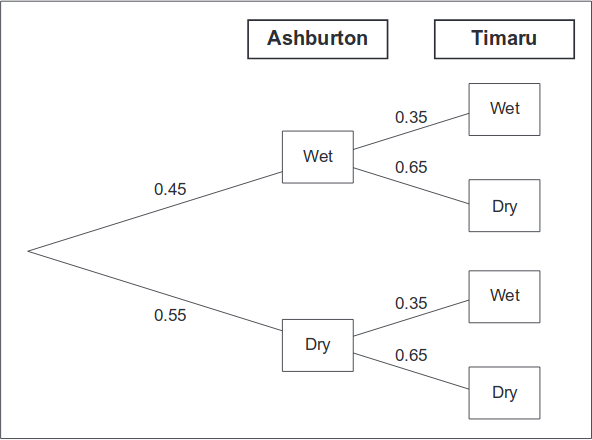
\includegraphics[width=0.4\textwidth]{treediagram}
            \end{center}
            Elain why Teri’s tree diagram would not give a correct answer to the probability that it is
            dry in both towns on the same day. (Note: the distance between Ashburton and Timaru is
            around \SI{75}{\kilo\metre}. Both towns lie on the Canterbury plains.)
    \end{parts}
  \fullwidth{\subsubsection*{Relative risk}}
  \question A study is conducted of 1500 randomly selected candidates for an international
            examination to investigate whether Y12 candidates are more successful than Y13
            candidates. The findings are summarised in the table below.

            \begin{center}
            \begin{tabular}{|c|c|c|c|}\hline
            & \textbf{Y12} & \textbf{Y13} & \textbf{Total}\\\hline
            \textbf{Pass} & 347 & 853 & 1200\\\hline
            \textbf{Fail} & 33 & 267 & 300\\\hline
            \textbf{Total} & 380 & 1120 & 1500\\\hline
            \end{tabular}
            \end{center}
    \begin{parts}
      \part What proportion of candidates passed the exam?
      \part What proportion of candidates who failed were in year 12?
      \part There were about 52\,500 candidates from year 12 and year 13
            who attempted the exam. Based on the results of the study, how many
            candidates would be expected to be in year 13 and pass the exam?
      \part It is claimed that year 13 candidates are four more times more likely
            to fail the exam than year 12 candidates. Discuss your agreement or
            disagreement with this statement.
    \end{parts}
  \question Polygraph (lie-detector) tests are often routinely administered to government
            employees or prospective employees in sensitive positions. A study performed in the US in 2002
            found that lie detector results are ``better than chance, but well below
            perfection''. Typically, the test will conclude someone is a spy 80\% of the time
            when he or she actually is a spy; but 16\% of the time, the test will conclude
            someone is a spy when he or she is not.
    \begin{parts}
      \part Assuming that 10 out of every 10\,000 employees are actual spies, compute the following:
        \begin{subparts}
          \subpart The probability that an employee is a spy and is ``detected'' to be one.
          \subpart The probability that an employee is \textbf{not} a spy and is ``detected'' to be one.
          \subpart The overall probability that the polygraph ``detects'' that an employee is a spy.
        \end{subparts}
      \part On the basis of the given information, and the probabilities that you have calculated,
            is the use of the polygraph ``worth it''?
    \end{parts}
  \question A survey was conducted in 2000, asking respondents about various driving habits. This table
            classifies 1\,086 participants according to type of car driven, and whether or not they were
            in the habit of making insulting gestures at other drivers.

            \begin{tabular}{|c|c|c|c|c|c|c|c|c|}\hline
            & \textbf{Economy} & \textbf{Family} & \textbf{Luxury} & \textbf{Sports} & \textbf{Truck} & \textbf{Utility} & \textbf{Van} & \textbf{Total}\\\hline
            \textbf{Gestures} & 79&65&16&58&42&32&8&300\\\hline
            \textbf{No Gestures} & 281&170&45&95&77&79&39&786\\\hline
            \textbf{Total} & 360&235&61&153&119&111&47&1086\\\hline
            \end{tabular}
    \begin{parts}
      \part Before calculating any conditional probabilities, identify the types of cars whose owners
            you would suspect to have a tendancy to make insulting gestures at other drivers.
      \part For each type of car, find the (conditional) probability that surveyed drivers of that type
            of car make insulting gestures (e.g. given that a person drives a truck, what is the probability
            that they make insulting gestures).
      \part Comment on whether your suspicions in part (a) were correct.
      \part To three decimal places each, find (using the table):
        \begin{subparts}
          \subpart The probability of driving a van ($P(V)$).
          \subpart The probability of making insulting gestures ($P(G)$).
          \subpart The probability of driving a van \textit{and} making insulting gestures ($P(V \cap G)$).
        \end{subparts}
      \part Check if $ P(V \cap G) = P(V) \times P(G) $ to see if the events $ V $ and $ G $ are independent. Explain the outcome.
      \part You found $ P(G | V) $ in part (b). Check if $ P(V \cap G) = P(V) \times P(G | V) $, and explain the outcome.
      \part Find the overall probability of driving an economy car, a family car, a luxury car, or a van.
      \part Find the probability of making insulting gestures, given that someone drives an economy car, a family car, a luxury car, or a van.
      \part Are drivers of economy cars, family cars, luxury cars, or vans less likely in general to make insulting gestures?
    \end{parts}
\end{questions}

\end{document}

